\documentclass[border=6pt]{standalone}
\usepackage[T1]{fontenc}
\usepackage{helvet}
\renewcommand\familydefault{\sfdefault}
\usepackage{tikz}
\usepackage{pgfplots}
\pgfplotsset{compat=1.18}
\usepackage{xcolor}

% Accent color: muted blue #1f4e79
\definecolor{accent}{rgb}{0.122,0.306,0.475}

\begin{document}
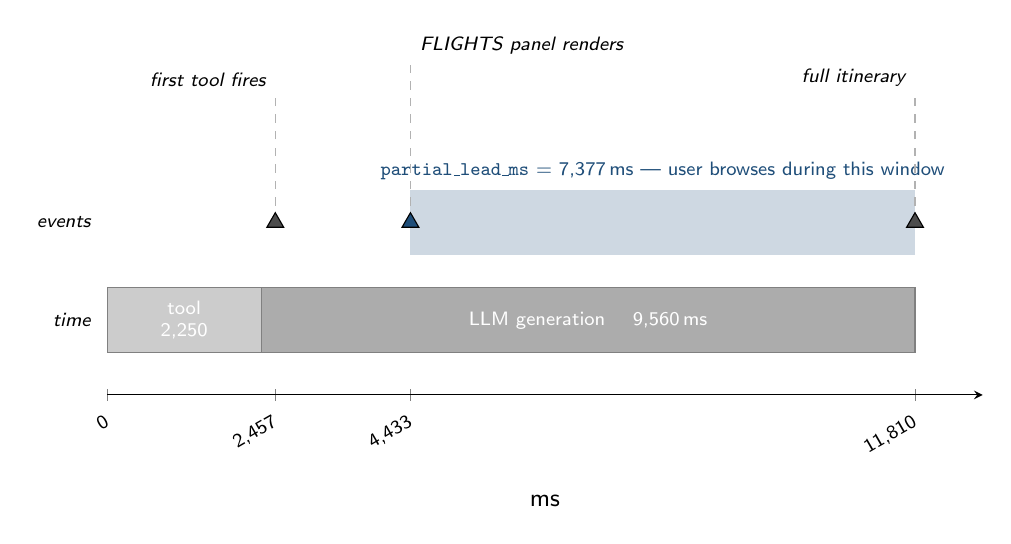
\begin{tikzpicture}[font=\small]
\begin{axis}[
  width=12.7cm,
  height=6.2cm,
  xmin=0, xmax=12800,
  ymin=0.1, ymax=4.0,
  axis x line=bottom,
  axis y line=none,
  % Four event-related ticks only (no axis-boundary tick that causes artifacts)
  xtick={0, 2457, 4433, 11810},
  xticklabels={0, 2{,}457, 4{,}433, 11{,}810},
  xticklabel style={font=\scriptsize, rotate=30, anchor=north east},
  ytick=\empty,
  xlabel={\small ms},
  xlabel style={at={(axis description cs:0.5,-0.25)}, anchor=north},
  clip=false,
  scaled x ticks=false,
]

%% ===== ROW 2 (y=0.55..1.25): Time-accounting horizontal bars =====
%% math: 2,250 + 9,560 = 11,810  (consistent with t_done tick)

% Tool execution bar: 0 → 2250  (pure TikZ rectangle avoids pgfplots ghost artifacts)
\filldraw[fill=gray!40, draw=black!50, line width=0.4pt]
  (axis cs:0,0.55) rectangle (axis cs:2250,1.25);

% LLM inference bar: 2250 → 11810
\filldraw[fill=gray!65, draw=black!50, line width=0.4pt]
  (axis cs:2250,0.55) rectangle (axis cs:11810,1.25);

% Labels inside bars
\node[font=\scriptsize, text=white, align=center]  at (axis cs:1125,0.90) {tool\\2,250};
\node[font=\scriptsize, text=white] at (axis cs:7030,0.90) {LLM generation \quad 9,560\,ms};

% Row label
\node[font=\scriptsize\itshape, anchor=east] at (axis cs:-100,0.90) {time};

%% ===== ROW 1 (y≈1.9): User-visible event markers =====

% Shaded partial_lead span: 4433 → 11810  (pure TikZ rectangle, no ghost artifacts)
\filldraw[fill=accent!22, draw=none]
  (axis cs:4433,1.60) rectangle (axis cs:11810,2.30);

% partial_lead label (above shade)
\node[font=\scriptsize, text=accent, anchor=south]
  at (axis cs:8121,2.30)
  {\texttt{partial\_lead\_ms}~=~7,377\,ms — user browses during this window};

% Row label
\node[font=\scriptsize\itshape, anchor=east] at (axis cs:-100,1.95) {events};

% Event markers: filled triangles (drawn as nodes, immune to axis distortion)
\addplot[mark=triangle*, mark size=3.5pt, mark options={fill=black!70, draw=none},
         only marks] coordinates {(2457,1.95)};
\addplot[mark=triangle*, mark size=3.5pt, mark options={fill=accent, draw=none},
         only marks] coordinates {(4433,1.95)};
\addplot[mark=triangle*, mark size=3.5pt, mark options={fill=black!70, draw=none},
         only marks] coordinates {(11810,1.95)};

%% ===== Event labels: staggered with vertical tick lines =====

% Thin dashed vertical lines from markers up to label row
\draw[black!30, thin, dashed] (axis cs:2457,1.95) -- (axis cs:2457,3.30);
\draw[black!30, thin, dashed] (axis cs:4433,1.95) -- (axis cs:4433,3.65);
\draw[black!30, thin, dashed] (axis cs:11810,1.95) -- (axis cs:11810,3.30);

% Labels: "first tool fires" right-of-center at 2457 (anchor south east = text left of point)
\node[font=\scriptsize\itshape, anchor=south east]
  at (axis cs:2457,3.30) {first tool fires};

% "FLIGHTS panel renders" at higher row (anchor south west = text right of point)
\node[font=\scriptsize\itshape, anchor=south west]
  at (axis cs:4433,3.65) {FLIGHTS panel renders};

% "full itinerary" (anchor south east = text left of point, avoids right clipping)
\node[font=\scriptsize\itshape, anchor=south east]
  at (axis cs:11810,3.30) {full itinerary};

\end{axis}
\end{tikzpicture}
\end{document}
